% GigaHack 2026 pitch in the organisers' template (GigaHack_2026_Pitch_Template.pptx), rebuilt in Beamer.
% Every box, label and font size is placed at the template's own coordinates: EMU / 76200 = mm on the
% 160 x 90 mm Beamer 16:9 page, pptx pt x 0.4724 = Beamer pt. Backgrounds and the logo are the template's images.
% Build: xelatex -output-directory=build gigahack.tex (twice: the boxes use remember picture).
\documentclass[aspectratio=169]{beamer}
\usepackage{fontspec}
\setsansfont{Arial}
\setmainfont{Arial}
\usepackage{tikz}
\setbeamertemplate{navigation symbols}{}
\setbeamertemplate{headline}{}
\setbeamertemplate{footline}{}

\definecolor{gGreen}{HTML}{00EF00}
\definecolor{gPurple}{HTML}{A68FFC}
\definecolor{gOrange}{HTML}{FF9F1C}
\definecolor{gBox}{HTML}{0C120E}
\definecolor{gBorder}{HTML}{2F4535}
\definecolor{gMuted}{HTML}{9AA5A0}
\definecolor{gDark}{HTML}{0A0A0A}

% background image of template slide N, plus the GigaHack logo bottom right (same on every slide)
\newcommand{\gbgnum}{3}
\newcommand{\bg}[1]{\renewcommand{\gbgnum}{#1}}
\setbeamertemplate{background}{%
  \begin{tikzpicture}[x=1mm,y=-1mm]
    \useasboundingbox (0,0) rectangle (160,90);
    \node[anchor=north west,inner sep=0] at (0,0) {\includegraphics[width=160mm,height=90mm]{media/Slide-\gbgnum-image-1.jpeg}};
    \node[anchor=north west,inner sep=0] at (120,82.2) {
\includegraphics[width=33.6mm,height=4.5mm]{media/image-2-2.png}};
  \end{tikzpicture}}

% pptx point size -> Beamer size (the page is 0.4724 of the pptx page)
\newcommand{\fs}[1]{\fontsize{\fpeval{round(#1*0.4724,2)}pt}{\fpeval{round(#1*0.4724*1.2,2)}pt}\selectfont}
% the template never hyphenates and uses single spaces after a full stop
\hyphenpenalty=10000
\exhyphenpenalty=10000
\AtBeginDocument{\frenchspacing}
\newcommand{\todo}[1]{\textcolor{gOrange}{[#1]}}

% canvas in template mm, origin top left, y down
\newenvironment{gslide}{\begin{tikzpicture}[remember picture,overlay,x=1mm,y=-1mm,shift={(current page.north west)}]}{\end{tikzpicture}}
% slide title (36 pt bold, white)
\newcommand{\gtitle}[1]{\node[anchor=west,inner sep=0,text=white,font={\fs{36}\bfseries}] at (6.6,10.5) {#1};}
% rounded card: x, y, w, h, border colour (0C120E at 88 %, 1.25 pt border, 1.44 mm corners)
\newcommand{\gbox}[5]{%
  \fill[gBox,fill opacity=.88,rounded corners=1.44mm] (#1,#2) rectangle ++(#3,#4);
  \draw[#5,line width=.59pt,rounded corners=1.44mm] (#1,#2) rectangle ++(#3,#4);}
% dashed green drop zone (demo, QR)
\newcommand{\gdbox}[4]{%
  \fill[gBox,fill opacity=.75,rounded corners=1.44mm] (#1,#2) rectangle ++(#3,#4);
  \draw[gGreen,line width=.71pt,dash pattern=on 2.1pt off 1.6pt,rounded corners=1.44mm] (#1,#2) rectangle ++(#3,#4);}
% 16 pt bold caps label, vertically centred in its 4.8 mm band: x, y, w, colour, text
\newcommand{\glab}[5]{\node[anchor=west,inner sep=0,text=#4,text width=#3mm,font={\fs{16}\bfseries}] at (#1,{#2+2.4}) {#5};}
% top-left text block: x, y, w, pptx size, text
\newcommand{\gtxt}[5]{\node[anchor=north west,inner sep=0,text=white,text width=#3mm,align=left,font={\fs{#4}}] at (#1,#2) {#5};}
% top-centred text block: x, y, w, pptx size, text
\newcommand{\gtxtc}[5]{\node[anchor=north,inner sep=0,text=white,text width=#3mm,align=center,font={\fs{#4}}] at ({#1+#3/2},#2) {#5};}
% big green number centred in a band: x, y, w, h, pptx size, text
\newcommand{\gbig}[6]{\node[anchor=center,inner sep=0,text=gGreen,font={\fs{#5}\bfseries}] at ({#1+#3/2},{#2+#4/2}) {#6};}
% numbered green disc: x, y (top left of the 6.6 mm disc), number
\newcommand{\gnum}[3]{\fill[gGreen] ({#1+3.3},{#2+3.3}) circle (3.3mm);
  \node[text=gDark,inner sep=0,font={\fs{18}\bfseries}] at ({#1+3.3},{#2+3.3}) {#3};}
% team card: x, name, role, one line, initials
\newcommand{\gcard}[5]{%
  \gbox{#1}{19.8}{27.6}{49.2}{gBorder}
  \fill[gBox,fill opacity=.7] ({#1+13.8},32.4) circle (9mm);
  \draw[gGreen,line width=.59pt,dash pattern=on 2.1pt off 1.6pt] ({#1+13.8},32.4) circle (9mm);
  \node[text=white,inner sep=0,font={\fs{24}\bfseries}] at ({#1+13.8},32.4) {#5};
  \gtxtc{#1+1.2}{43.8}{25.2}{18}{\bfseries #2}
  \node[anchor=north,inner sep=0,text=gGreen,text width=25.2mm,align=center,font={\fs{15}}] at ({#1+13.8},51.6) {#3};
  \gtxtc{#1+1.2}{56.4}{25.2}{13}{#4}}

\begin{document}

% ---------------------------------------------------------------- 1 · title + hook (0:15)
\bg{2}
\begin{frame}[plain]
\begin{gslide}
  \node[anchor=north west,inner sep=0] at (8.4,8.4) {
\includegraphics[width=48mm,height=3.6mm]{media/image-2-3.png}};
  \node[anchor=west,inner sep=0,text=gGreen,font={\fs{60}\bfseries}] at (8.4,26.4) {Solemtrix Vineyard AI};
  \gtxt{8.4}{35.4}{126}{22}{For vineyard inspectors and farmers who can't check every vine on foot, we built an offline AI pipeline and web map that turns one drone flight into a per-plant inventory and a 25\,km inspection walk.}
  \gbox{8.4}{54}{142.8}{22.8}{gBorder}
  \glab{12}{56.6}{48}{gPurple}{CHALLENGE}
  \gtxt{12}{61.2}{74.4}{16}{AI/ML · AgriFood · GeoTech — Vineyard AI Field Challenge (Sireț3) — Marcaj}
  \glab{91.2}{56.6}{48}{gPurple}{TEAM}
  \gtxt{91.2}{61.2}{57.6}{16}{Solemtrix Hardware \& Software — Miroslav Maletici, Razvan Pervulescu, \todo{other members}}
\end{gslide}
\end{frame}

% ---------------------------------------------------------------- 2 · the problem (0:45)
\bg{3}
\begin{frame}[plain]
\begin{gslide}
  \gtitle{The problem}
  \gbox{6.6}{19.2}{91.2}{58.8}{gBorder}
  \glab{10.2}{22.2}{84}{gGreen}{WHO HAS THIS PROBLEM?}
  \gtxt{10.2}{27.6}{84}{18}{State vineyard inspectors (vine registry, subsidy checks), farmers and agronomists who need to know every row and every plant.}
  \glab{10.2}{39.6}{84}{gGreen}{WHAT HAPPENS TODAY?}
  \gtxt{10.2}{45}{84}{18}{An inspector walks every inter-row: 68\,km and $\approx$\,17\,h for the 81.5\,ha of Sireț3, and still has no per-plant record of gaps, missing vines or waste.}
  \glab{10.2}{57}{84}{gGreen}{WHY DOES IT MATTER TO THE CHALLENGE PROVIDER?}
  \gtxt{10.2}{62.4}{84}{18}{Aerial images alone give no measured areas and no efficient walking plan, while the registry (45,500\,ha) and statistics (66,400\,ha) differ by 20,900\,ha.}
  \gbox{101.4}{19.2}{52}{58.8}{gGreen}
  \gbig{101.4}{26.4}{52}{19.2}{66}{17 h}
  \gtxtc{105.6}{48}{43.8}{16}{on foot to inspect one 81.5\,ha village: a 68\,km serpentine through every inter-row}
\end{gslide}
\end{frame}

% ---------------------------------------------------------------- 3 · our solution (with the demo: 2:00)
\bg{4}
\begin{frame}[plain]
\begin{gslide}
  \gtitle{Our solution}
  \gbox{6.6}{19.2}{146.8}{18.6}{gGreen}
  \node[anchor=west,inner sep=0,text=white,text width=139.2mm,font={\fs{20}}] at (10.8,28.5) {One drone flight in: every vineyard block, row and plant measured with an ID, checked in Marcaj, and the shortest closed inspection walk out. Offline, on one laptop, in $\approx$\,17 minutes.};
  \gbox{6.6}{41.4}{47.4}{36.6}{gBorder}
  \gnum{10.2}{44.4}{1}
  \gtxt{10.2}{53.4}{40.2}{20}{\bfseries Per-plant map}
  \gtxt{10.2}{60.6}{40.2}{16}{Click any block, row, plant or waste spot and see its ID and attributes: 674 rows, 13,702 plants.}
  \gbox{56.3}{41.4}{47.4}{36.6}{gBorder}
  \gnum{59.9}{44.4}{2}
  \gtxt{59.9}{53.4}{40.2}{20}{\bfseries Measurements}
  \gtxt{59.9}{60.6}{40.2}{16}{Counts, row lengths, canopy and inter-row areas per block and farm, tied to cadastre parcels.}
  \gbox{106}{41.4}{47.4}{36.6}{gBorder}
  \gnum{109.6}{44.4}{3}
  \gtxt{109.6}{53.4}{40.2}{20}{\bfseries Inspection route}
  \gtxt{109.6}{60.6}{40.2}{16}{Walk, or send a robot, along a closed 25\,km route through 790 targets; GPX per farm.}
\end{gslide}
\end{frame}

% ---------------------------------------------------------------- 4 · demo
\bg{5}
\begin{frame}[plain]
\begin{gslide}
  \gtitle{Demo}
  \gdbox{6.6}{19.2}{146.8}{58.8}
  \node[anchor=north west,inner sep=0] at (9.6,21.6) {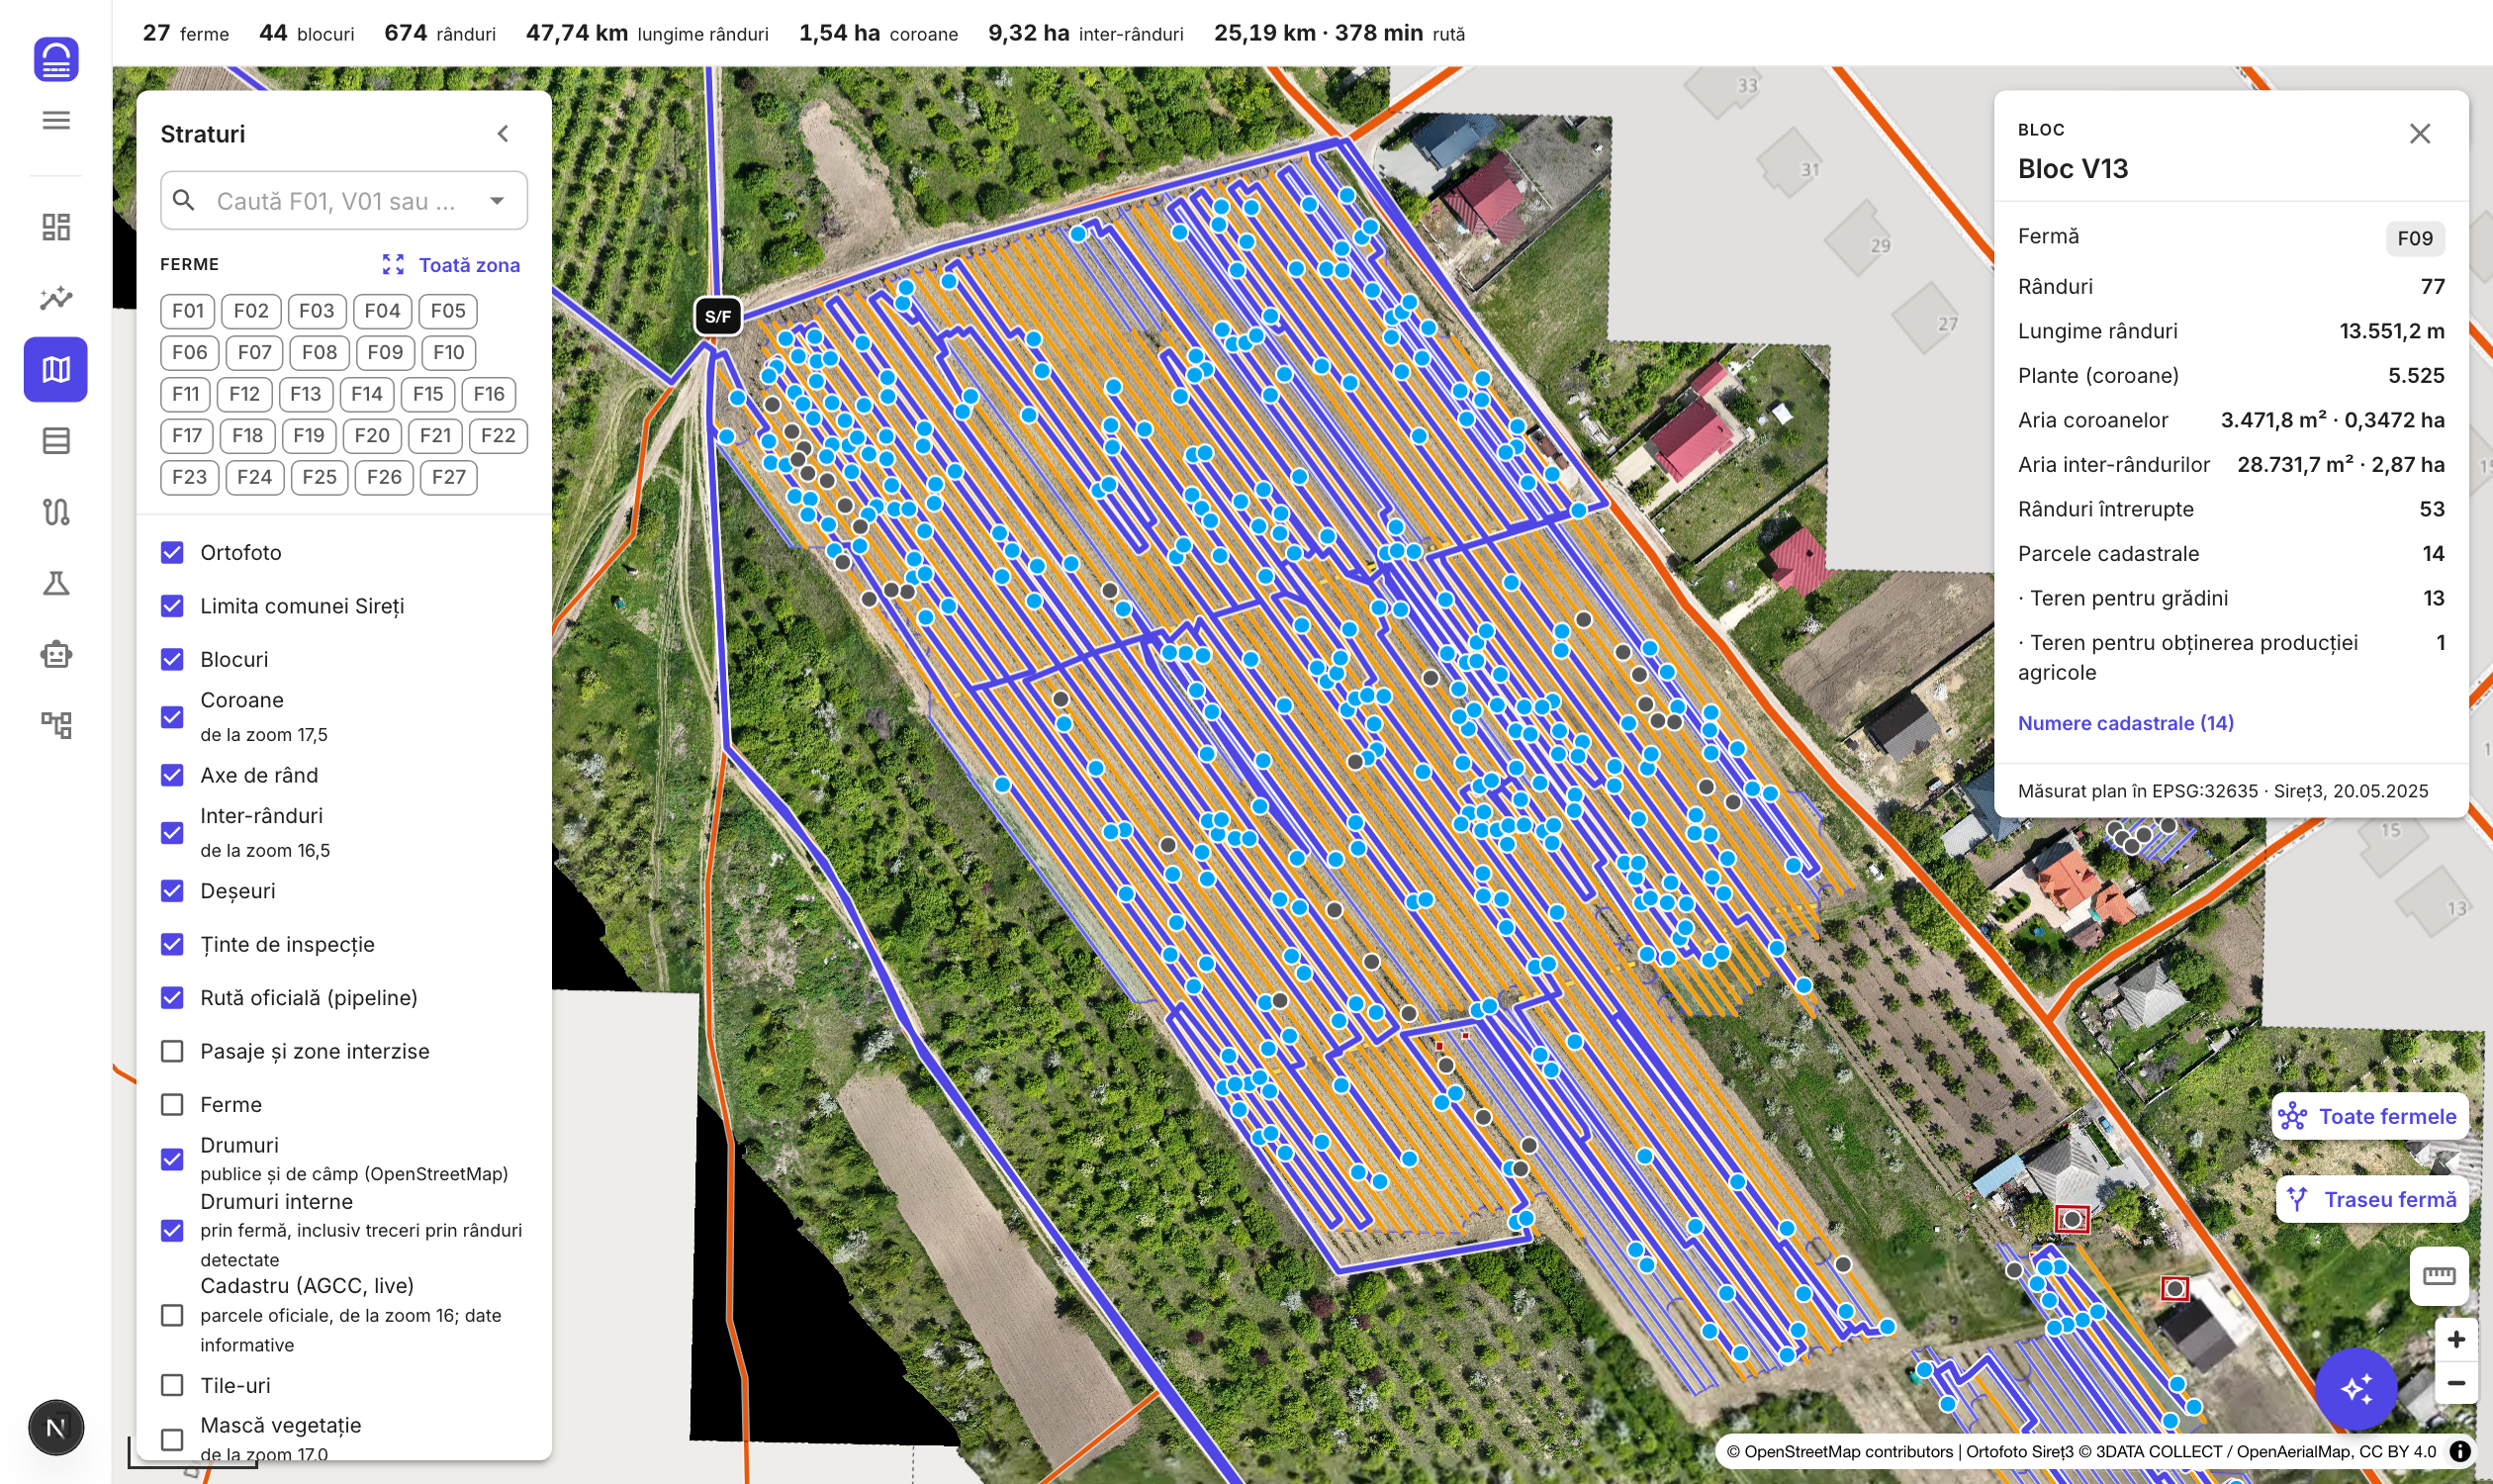
\includegraphics[width=90.7mm,height=54mm]{img/demo_map.png}};
  \gtxt{104.4}{23.4}{46}{16}{\textcolor{gGreen}{\bfseries SCREENCAST}\\[0.6mm]\todo{YouTube link}}
  \gtxt{104.4}{35.4}{46}{16}{\textcolor{gGreen}{\bfseries ONE USER, ONE TASK}\\[0.6mm]An inspector opens farm F09, block V13, row V13-R020: counts, areas, gaps, then the route as GPX.}
  \gtxt{104.4}{56.4}{46}{16}{\textcolor{gGreen}{\bfseries PRE-TEST POINT}\\[0.6mm]47.1225\,N, 28.7095\,E: block V13, inter-row V13-I020; our route passes 0.34\,m away.}
\end{gslide}
\end{frame}

% ---------------------------------------------------------------- 5 · how it works (0:45)
\bg{6}
\begin{frame}[plain]
\begin{gslide}
  \gtitle{How it works}
  \gbox{6.6}{19.8}{43.2}{28.8}{gBorder}
  \glab{10.2}{22.2}{36}{gPurple}{INPUT}
  \gtxt{10.2}{28.2}{36}{16}{311 drone GeoTIFFs (2.5\,cm/px, 81.5\,ha, EPSG:32635), AGCC cadastre, OSM roads. Only 2 labelled tiles.}
  \node[inner sep=0,text=gGreen,font={\fs{36}\bfseries}] at (54.1,34.2) {→};
  \gbox{58.4}{19.8}{43.2}{28.8}{gGreen}
  \glab{62}{22.2}{36}{gGreen}{OUR ENGINE}
  \gtxt{62}{28.2}{36}{16}{CV first: rows as a 1-D signal, one canopy per plant, rule-based attributes; U-Net on 88 tiles; waste cascade; OR-Tools route.}
  \node[inner sep=0,text=gGreen,font={\fs{36}\bfseries}] at (105.9,34.2) {→};
  \gbox{110.3}{19.8}{43.2}{28.8}{gBorder}
  \glab{113.9}{22.2}{36}{gPurple}{OUTPUT}
  \gtxt{113.9}{28.2}{36}{16}{Marcaj annotations, measurements.csv, route GeoJSON / GPX, a web map with every ID (RO / EN / RU).}
  \gbox{6.6}{52.2}{72}{25.8}{gBorder}
  \glab{10.2}{54.6}{60}{gGreen}{WHAT'S REAL}
  \gtxt{10.2}{60}{64.8}{16}{The full flow on all 311 real tiles in $\approx$\,17 min on one laptop CPU, no paid API. On the 2 labelled tiles: row F1 1.00, canopy 0.876, inter-row IoU 0.96.}
  \gbox{81.4}{52.2}{72}{25.8}{gBorder}
  \glab{85}{54.6}{60}{gOrange}{WHAT'S STILL MOCKED}
  \gtxt{85}{60}{64.8}{16}{A human still checks every tile in Marcaj. The robot is a prototype on sample panoramas. Registry / AIPA export is not built. Deployment hours are estimates.}
\end{gslide}
\end{frame}

% ---------------------------------------------------------------- 6 · impact (with next steps: 0:45)
\bg{7}
\begin{frame}[plain]
\begin{gslide}
  \gtitle{Impact}
  \gbox{6.6}{19.8}{47.4}{33.6}{gGreen}
  \gbig{6.6}{22.2}{47.4}{15.6}{54}{−63\,\%}
  \gtxtc{10.2}{39.6}{40.2}{16}{shorter inspection walk: 25.2\,km instead of a 68.2\,km serpentine}
  \gbox{56.3}{19.8}{47.4}{33.6}{gBorder}
  \gbig{56.3}{22.2}{47.4}{15.6}{54}{10.7 h}
  \gtxtc{59.9}{39.6}{40.2}{16}{inspector time saved per survey: 6.3\,h instead of 17\,h}
  \gbox{106}{19.8}{47.4}{33.6}{gBorder}
  \gbig{106}{22.2}{47.4}{15.6}{54}{17 min}
  \gtxtc{109.6}{39.6}{40.2}{16}{from 311 tiles to deliverables on one laptop CPU, no paid API}
  \gbox{6.6}{56.4}{146.8}{21.6}{gBorder}
  \glab{10.2}{58.8}{132}{gGreen}{WHAT THIS MEANS FOR THE CHALLENGE PROVIDER}
  \gtxt{10.2}{64.2}{139.2}{17}{Marcaj's users get measured areas and an efficient walk, not just pictures. Deployment takes $\approx$\,11–20\,h from zero to the first inspected region: 6–11\,h one-time setup, then 5–9\,h per survey, mostly the human check. Route and compute are measured on Sireț3 at 4\,km/h; setup hours are estimates.}
\end{gslide}
\end{frame}

% ---------------------------------------------------------------- 7 · next steps and scaling
\bg{8}
\begin{frame}[plain]
\begin{gslide}
  \gtitle{Next steps}
  \draw[gGreen,line width=.94pt] (15.6,27.6) -- (114,27.6);
  \foreach \x in {12,61.2,110.4} {\fill[gGreen] ({\x+3.6},27.6) circle (3.6mm); \draw[gDark,line width=1.4pt] ({\x+3.6},27.6) circle (3.6mm);}
  \glab{9.6}{34.2}{43.2}{gPurple}{NEXT WEEK}
  \gtxt{9.6}{39.6}{42}{16}{Run a second village from the next drone flight; export results per cadastre parcel for the vine registry.}
  \glab{58.8}{34.2}{43.2}{gPurple}{NEXT MONTH}
  \gtxt{58.8}{39.6}{42}{16}{Season-to-season change per row; an offline Docker image for ministry servers; per-farm GPX and CSV reports.}
  \glab{108}{34.2}{43.2}{gPurple}{IN 3 MONTHS}
  \gtxt{108}{39.6}{42}{16}{A ground robot drives our route: side cameras, on-board disease detection, every image tied to its row\_id.}
  \gbox{6.6}{58.2}{146.8}{19.8}{gBorder}
  \glab{10.2}{60.6}{132}{gGreen}{WHAT WE NEED · HOW IT SCALES}
  \gtxt{10.2}{66}{139.2}{17}{More flights and 2 labelled tiles per region, and a pilot with the vine registry (ONVV) and AIPA. Measured 4.7\,s/ha: all $\approx$\,100,000\,ha of Moldovan vineyards in $\approx$\,130\,h on one laptop, $\approx$\,16\,h on a 64-core server (extrapolated).}
\end{gslide}
\end{frame}

% ---------------------------------------------------------------- 8 · team (with the close: 0:30)
\bg{9}
\begin{frame}[plain]
\begin{gslide}
  \gtitle{Team}
  \gcard{36.4}{Miroslav\\Maletici}{AI \& pipeline}{CV pipeline, U-Net, route solver, Marcaj export}{MM}
  \gcard{66.1}{Razvan\\Pervulescu}{Web platform}{Map, statistics, farm routes, robot views}{RP}
  \gcard{95.9}{\todo{Name}}{\todo{Role}}{\todo{One line: why you}}{?}
  \node[anchor=north west,inner sep=0,text=gMuted,font={\fs{14}}] at (6.6,72) {Team lead: \todo{name}. Solemtrix Hardware \& Software.};
\end{gslide}
\end{frame}

% ---------------------------------------------------------------- 9 · thank you
\bg{10}
\begin{frame}[plain]
\begin{gslide}
  \node[anchor=west,inner sep=0,text=white,text width=142.8mm,font={\fs{32}}] at (8.4,28.8) {One drone flight: every vine measured with an ID, and a 25\,km walk instead of 68\,km. Offline, on one laptop, in 17 minutes.};
  \node[anchor=west,inner sep=0,text=gGreen,font={\fs{48}\bfseries}] at (8.4,51.6) {Thank you!};
  \gtxt{8.4}{58.8}{102}{18}{Solemtrix Hardware \& Software · \todo{email / LinkedIn}\\github.com/miroslav43/Solemtrix\_Hardware\_Software\_\_\\Vineyard\_AI\_Field\_Challenge}
  \gdbox{121.2}{45}{30}{30}
  \node[inner sep=0] at (136.2,60) {
\includegraphics[width=25mm]{img/qr_repo.png}};
\end{gslide}
\end{frame}

% ================================================================ backup
\bg{11}
\begin{frame}[plain]
\begin{gslide}
  \node[anchor=west,inner sep=0,text=gGreen,font={\fs{54}\bfseries}] at (8.4,37.8) {Backup slides};
  \node[anchor=west,inner sep=0,text=white,font={\fs{22}}] at (8.4,48.6) {Not part of the 5 minutes. Show them only if the jury asks.};
\end{gslide}
\end{frame}

\bg{12}
\begin{frame}[plain]
\begin{gslide}
  \gtitle{Backup: details for Q\&A}
  \gbox{6.6}{19.8}{71.4}{58.2}{gBorder}
  \glab{10.2}{22.8}{64.2}{gGreen}{TECHNICAL DETAILS}
  \gtxt{10.2}{28.8}{64.2}{15}{%
    \textbf{Rows:} dominant angle, 1-D projection, autocorrelation spacing (1.8–3.8\,m), SNR\,$\geq$\,3 rejects orchards, Huber fit, union-find across tiles.\\[0.8mm]
    \textbf{Canopies:} Lab a* threshold inside the row corridor, one polygon per plant; U-Net only on 88 tiles (13\,s).\\[0.8mm]
    \textbf{Waste:} colour and shape rules, OpenCLIP probe, SAM\,3 on the top crops; a human approves every box.\\[0.8mm]
    \textbf{Route:} walking graph on inter-rows and authorised passages, generalised TSP (OR-Tools, 2-opt), closed at START, 1.23\,\% outside.\\[0.8mm]
    \textbf{2 labelled tiles:} row F1 1.00 (51/51), canopy 0.876, inter-row IoU 0.96, counts 0.973.\\[0.8mm]
    \textbf{Engineering:} $\approx$\,17 min on an Apple M3 Pro CPU; 2,378 tests, CI, offline Docker.}
  \gbox{82}{19.8}{71.4}{58.2}{gBorder}
  \glab{85.6}{22.8}{64.2}{gGreen}{BUSINESS / SUSTAINABILITY}
  \gtxt{85.6}{28.8}{64.2}{15}{%
    \textbf{Who would pay:} the vine registry and AIPA per surveyed hectare for subsidy checks; farms and cooperatives per survey for replanting and clean-up maps; a robot service per inspected row.\\[0.8mm]
    \textbf{Cost per survey:} no paid API, no GPU, open weights. What remains is the drone flight and 4–8\,h of human checking in Marcaj.\\[0.8mm]
    \textbf{Keeps running:} one config file, a pinned uv.lock and an offline Docker image (\texttt{--network none}) on government servers; the web app in RO / EN / RU.}
\end{gslide}
\end{frame}

\begin{frame}[plain]
\begin{gslide}
  \gtitle{Backup: the organisers' pre-test point}
  \gbox{6.6}{19.8}{92.4}{58.2}{gBorder}
  \node[anchor=north west,inner sep=0] at (9.6,23.4) {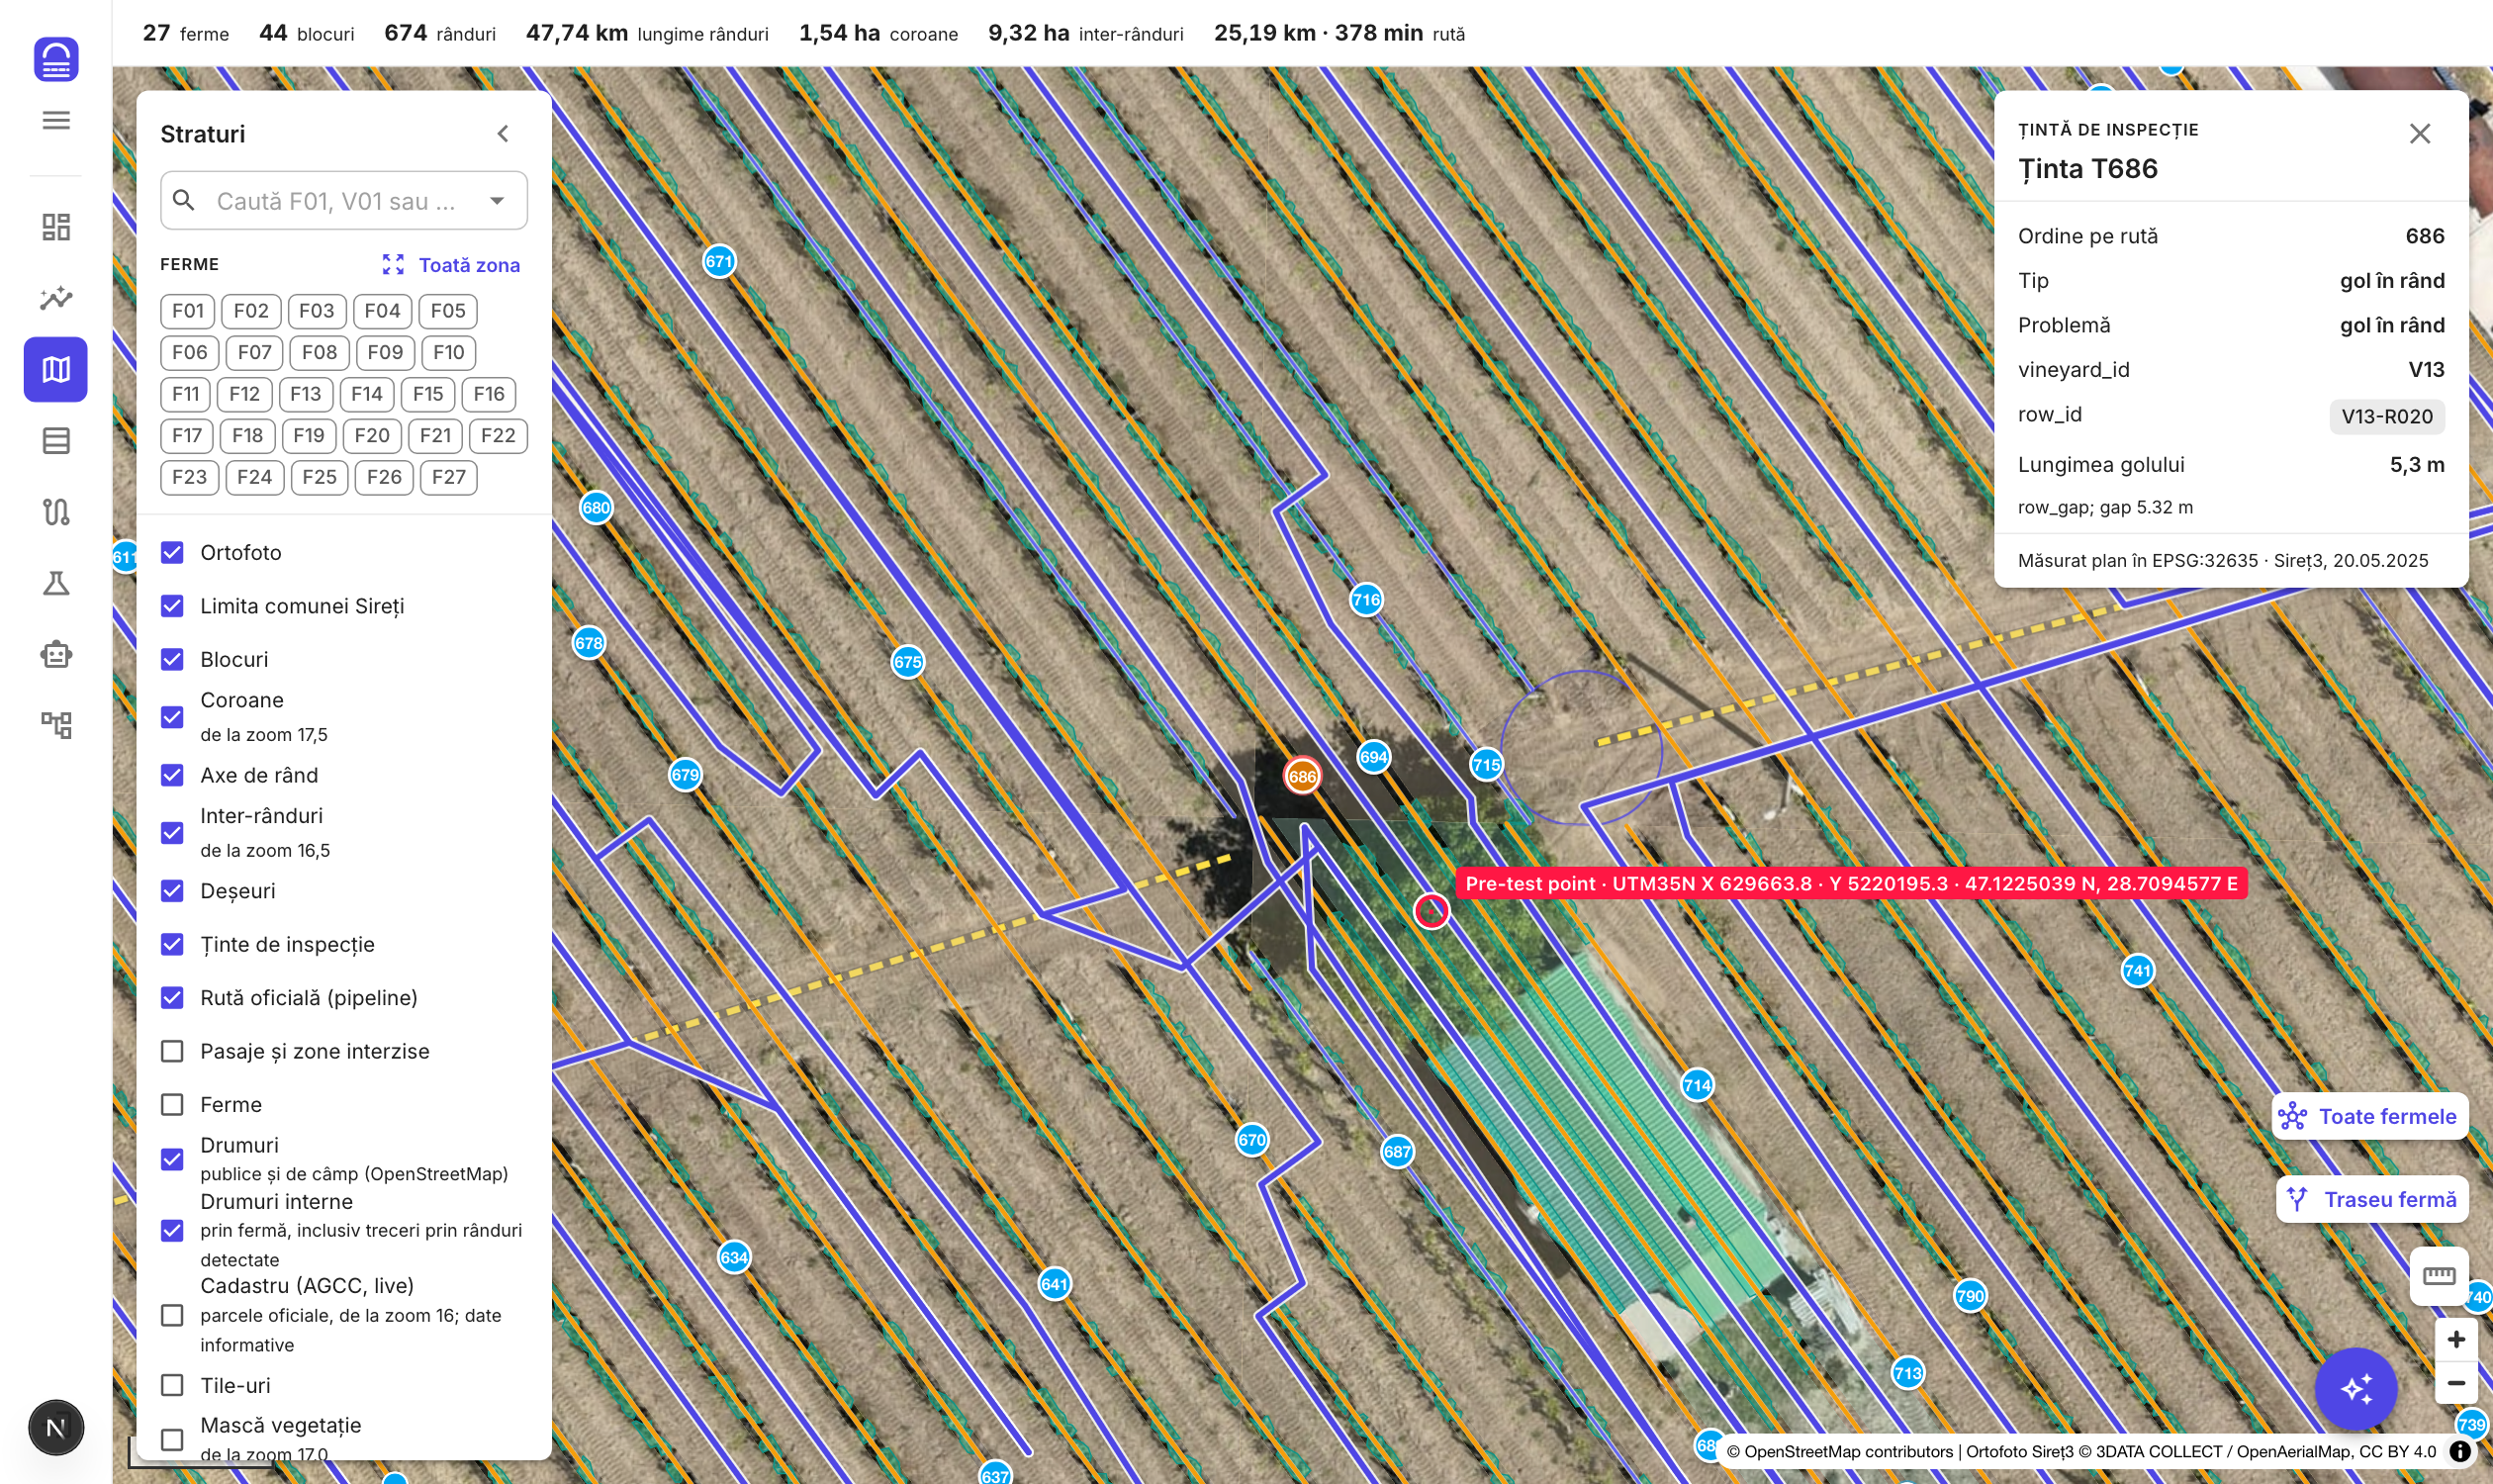
\includegraphics[width=86.4mm,height=51.4mm]{img/pretest_map.png}};
  \gbox{102}{19.8}{51.4}{58.2}{gGreen}
  \glab{105.6}{22.8}{45}{gGreen}{X 629663.8 · Y 5220195.3}
  \gtxt{105.6}{28.8}{45}{15}{%
    EPSG:32635 = 47.1225039\,N, 28.7094577\,E\\[0.8mm]
    \textbf{Tile} siret3\_r020\_c013\\
    \textbf{Farm / block} F09 / V13 (14 parcels)\\
    \textbf{Object} inter-row V13-I020, \emph{mixed}\\
    \textbf{Rows} V13-R020 at 0.82\,m (\emph{disrupted}, 228.94\,m, 70 plants), V13-R019 at 1.43\,m\\[0.8mm]
    \textbf{Route} passes 0.34\,m away: visited ($\leq$\,2\,m)\\
    \textbf{Block V13} 77 rows, 13,551\,m, canopy 3,472\,m², inter-row 28,732\,m²}
\end{gslide}
\end{frame}

\begin{frame}[plain]
\begin{gslide}
  \gtitle{Backup: deployment time, 11–20 h}
  \gbox{6.6}{19.8}{71.4}{58.2}{gBorder}
  \glab{10.2}{22.8}{64.2}{gGreen}{ONE-TIME SETUP · 6–11 H}
  \gtxt{10.2}{28.8}{64.2}{16}{%
    \begin{tabular}{@{}p{52mm}@{\hspace{2mm}}r@{}}
    Server or laptop: Docker or \texttt{uv sync}, \texttt{pnpm install}, model weights from the GitHub release & 1–2\,h\\[1.5mm]
    Web app for inspectors: build, hosting, TLS, logins & 2–3\,h\\[1.5mm]
    Calibrate a new region: label 2 reference tiles, check the thresholds & 2–4\,h\\[1.5mm]
    Train the operators (inspector, agronomist) & 1–2\,h
    \end{tabular}}
  \gbox{82}{19.8}{71.4}{58.2}{gBorder}
  \glab{85.6}{22.8}{64.2}{gGreen}{PER NEW SURVEY (≈ 80 HA) · 5–9 H}
  \gtxt{85.6}{28.8}{64.2}{16}{%
    \begin{tabular}{@{}p{52mm}@{\hspace{2mm}}r@{}}
    Ingest and AI pipeline (measured: 2.5\,s + $\approx$\,17 min) & 0.5\,h\\[1.5mm]
    Human check in Marcaj & 4–8\,h\\[1.5mm]
    Final run: route, measurements, reports, publish & 0.5\,h
    \end{tabular}\\[4mm]
    \textcolor{gMuted}{Compute times are measured (README §6). Setup and human-check times are team estimates.}}
\end{gslide}
\end{frame}

\end{document}
